\headline{{\textbf{\Large\sffamily TWBC Workshops:}}\\
          {\textbf{\large\sffamily A Great Success for Our First MEP Day}}}
\label{2025-12-workshop-mep}

\topic{The Birth of a New Tradition}
\noindent
Following the initial proposal back in August, the Member Education Programme (MEP) has officially transitioned from a promising concept to a vibrant reality. The initiative was born out of a desire to bridge the gap between watching demonstrations and hands-on practice. The response from the membership was immediate and overwhelming, with 19 members voting in favour of the launch. This enthusiasm has translated directly into bookings; since opening the registrations, seats for the scheduled sessions have been snapped up almost instantly, proving that there is a significant appetite within the Twickenham Bonsai Club for structured, mentor-led learning.

The MEP is designed specifically to support our novice members by pairing them with more experienced practitioners. By providing a dedicated space and time, the club ensures that the "Twickenham family" spirit continues to thrive, passing down years of collective wisdom in a focused environment.

\medskip
\topic{A Saturday Morning at Whitton}
\noindent
On Saturday, 13th December, the Whitton Community Centre’s front room was transformed into a bustling bonsai studio for our inaugural session. Transitioning from our usual Thursday evening meetings to a Saturday morning proved to be a masterstroke of convenience. Avoiding the post-work rush allowed for a refreshed start, and the atmosphere was noticeably different—relaxed, yet buzzing with intent.

Upon arrival, I found the space perfectly organised. Large tables were set up, providing ample room for each participant to spread out their tools and trees. The theme for the morning was \textbf{winter structural pruning and wiring}. Tony Ulatowski and Chris Durne led the session, moving methodically between the tables. Their approach was particularly commendable: they began by listening. Each participant had the opportunity to explain their tree’s history and their goals before receiving a tailored array of advice.

The technical guidance was profound. We moved beyond simple aesthetics, diving deep into the physiology of the trees. Suggestions ranged from bold structural choices—removing major branches to improve the silhouette—to advanced techniques like double-wiring trunks for heavy bends or using guy wires to set long-term development. Senior members, including Terry and Tina, worked on their own trees while simultaneously offering a helping hand to others, creating a seamless flow of mentorship.

\medskip
\topic{Personal Reflections: More Than Just Pruning}
\noindent
As I worked on my own trees, I felt a genuine shift in my understanding of the craft. It wasn't just about where to cut, but why. The "fear factor" that often haunts novice growers began to dissipate, replaced by a sense of calculated confidence. I managed to bring along my dog, who would have otherwise spent the morning howling at home—a small but significant detail that highlights the welcoming, community-oriented nature of these Saturday sessions.

In my view, the MEP represents the very best of TWBC. It is an investment in the members themselves. By covering the venue costs, the club has removed the barriers to entry, allowing us to focus entirely on the art. I left the session feeling that I had made more progress in three hours than I might have in months of solitary practice.

\end{multicols}
\vspace*{2em}
\begin{minipage}[b]{1.0\textwidth}
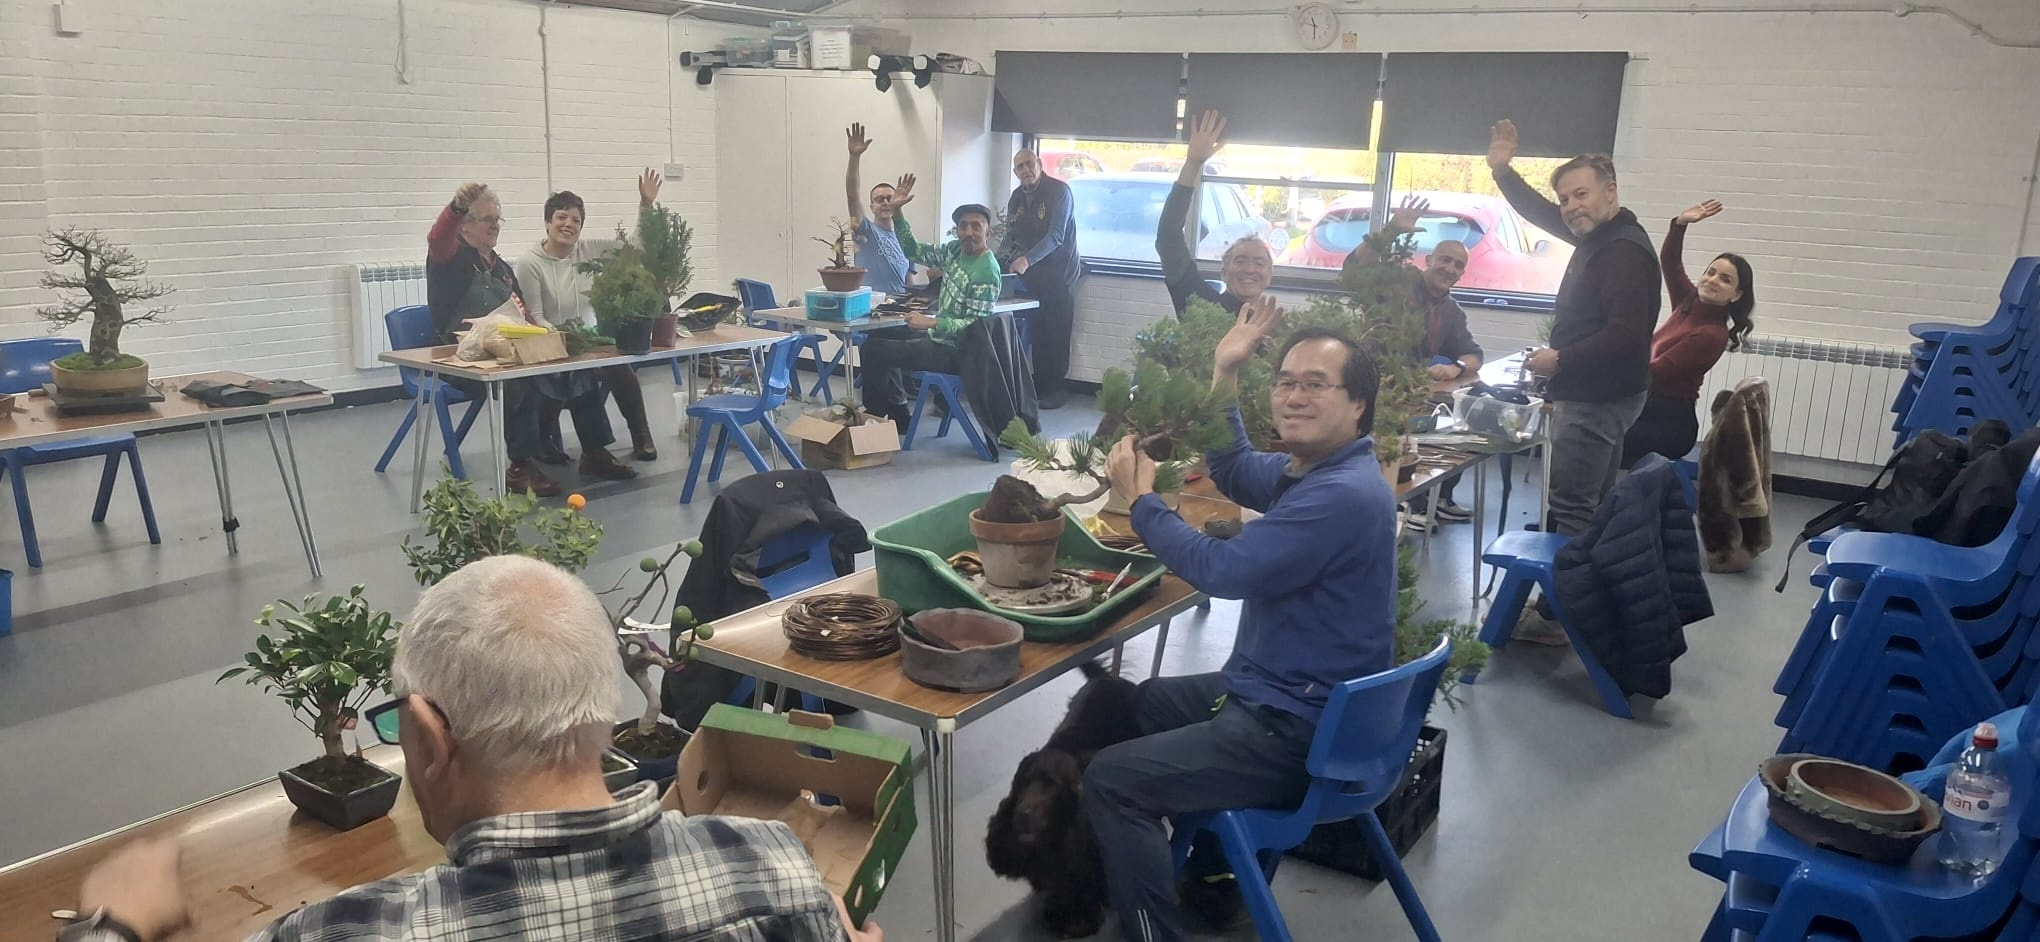
\includegraphics[angle=0,origin=c,width=1.0\textwidth]{2025_12/res/workshop-mep-opening}
\centerline{\emph{The buzzing atmosphere and camaraderie during TWBC's first MEP workshop.}}
\end{minipage}
\medskip
\begin{multicols}{2}

\begin{minipage}[b]{0.45\textwidth}
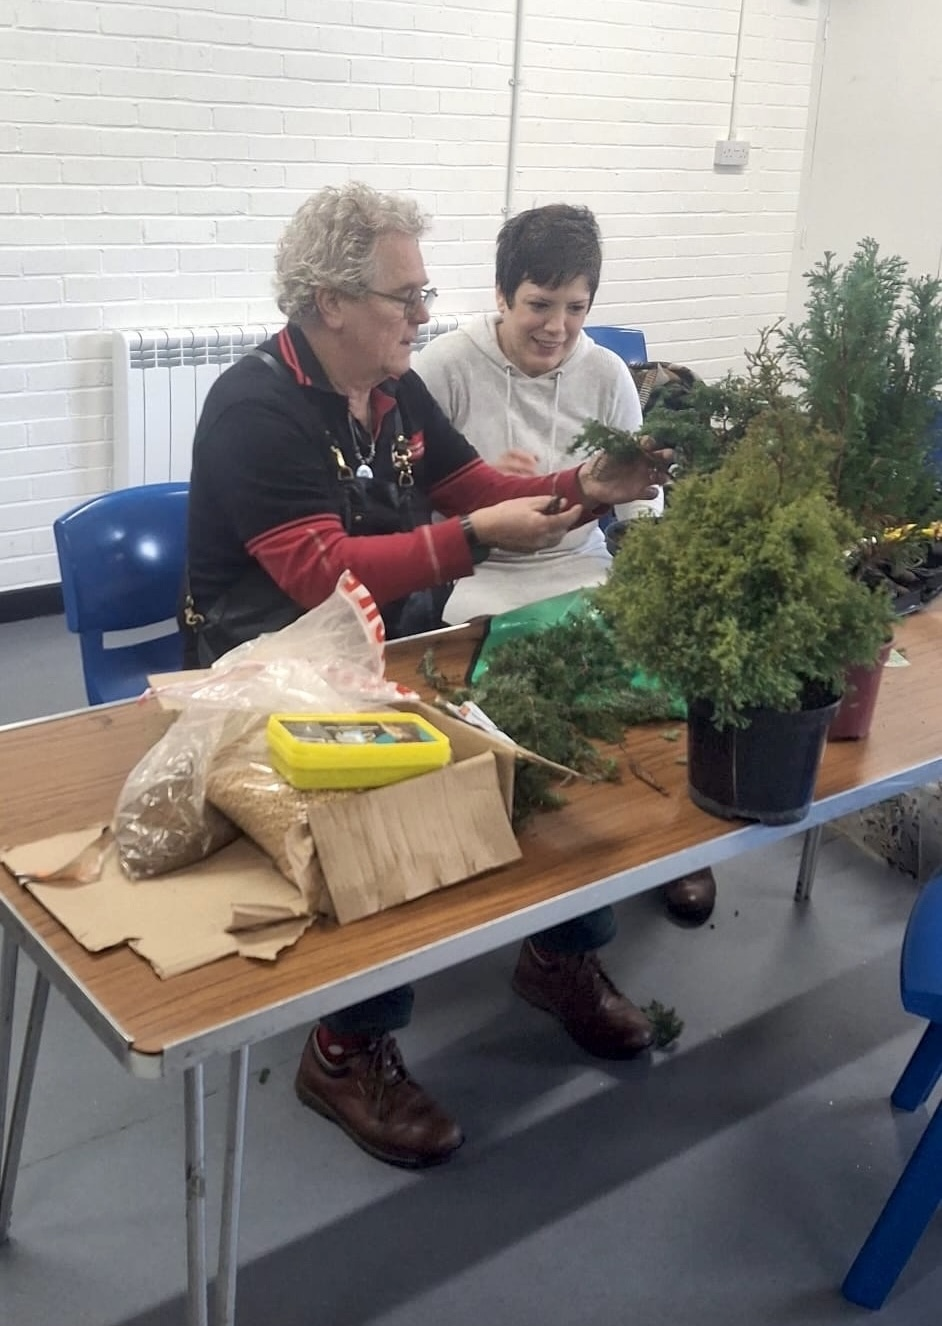
\includegraphics[angle=0,origin=c,width=1.0\textwidth]{2025_12/res/workshop-mep-ulatowski}
\centerline{\emph{Tony Ulatowski guiding a member on winter pruning.}}
\end{minipage}

\begin{minipage}[b]{0.45\textwidth}
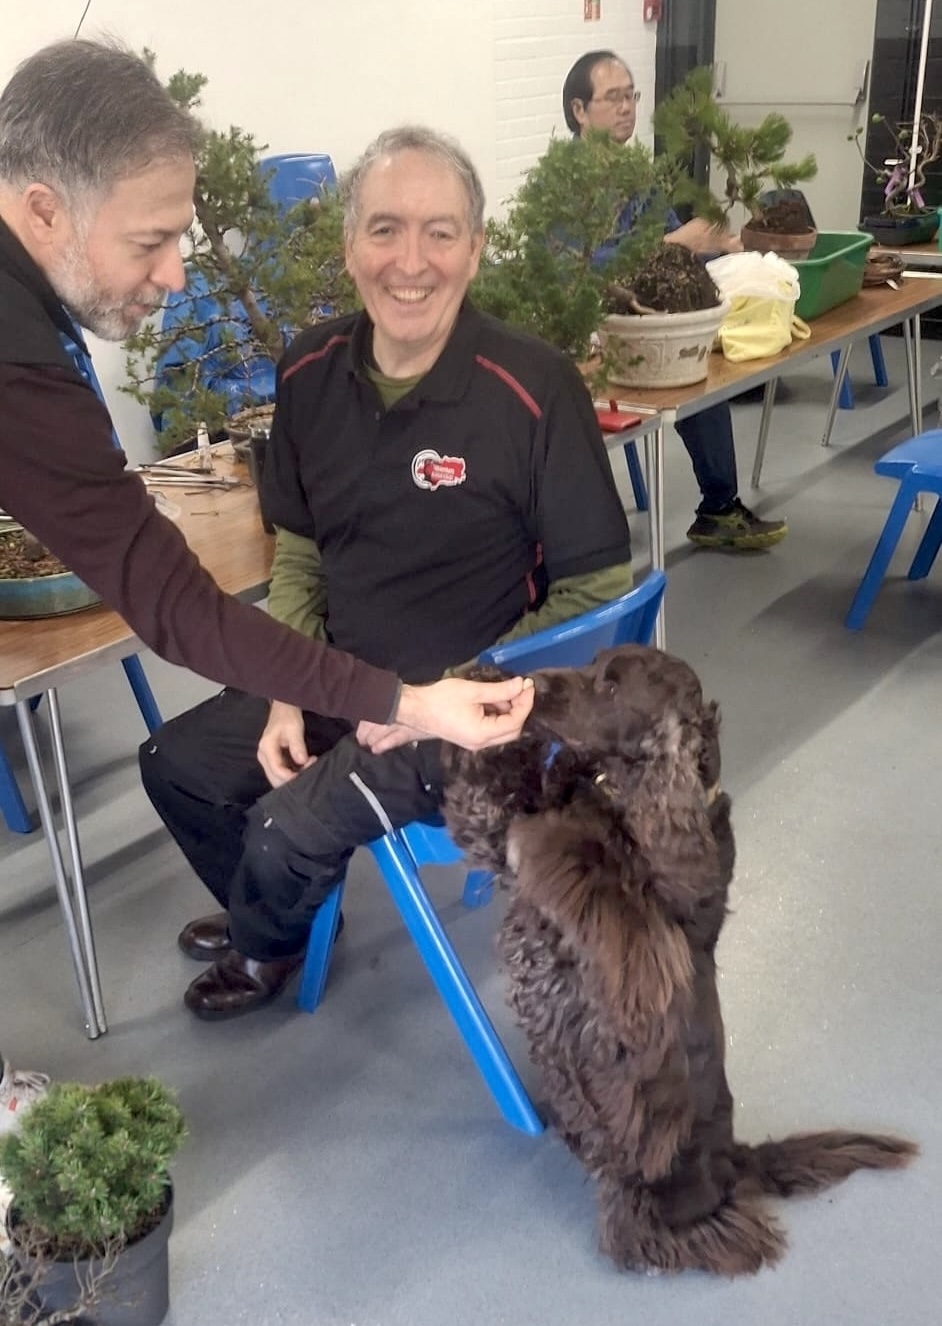
\includegraphics[angle=0,origin=c,width=1.0\textwidth]{2025_12/res/workshop-mep-durne}
\centerline{\emph{Chris Durne and a furry visitor enjoy the morning.}}
\end{minipage}

\medskip
\topic{Voices from the Bench: Member Feedback}
\noindent
The sentiment across the room was echoed in the feedback received after the event. \textbf{John Mari} noted: \emph{"It's brilliant having guest speakers, but you can’t beat working on your own trees and being guided by experts to really learn. I genuinely would love it to continue."}

For many, the psychological boost was as important as the technical one. \textbf{Riz Mizra} shared: \emph{"Unlike other workshops, you don't feel silly asking weird questions. I got a great buzz from today!"} Similarly, \textbf{Martin Redfern} commented on the impact on his self-belief: \emph{"As someone who suffers with lack of confidence and vision, it really helped today to build a bit more positivity into my way of thinking about my abilities."} \textbf{Tina Todd} summed up the morning perfectly, asking: \emph{"Where did 3 hours go? I've gained a lot of confidence today."}

\medskip
\topic{From the Organisers: A Positive Template}
\noindent
The organisers were equally encouraged by the turnout and the quality of work produced. \textbf{Chris Durne} remarked on the standard of the club: \emph{"No wonder TWBC is the best bonsai club in London with so many willing and able members."}

\textbf{Tony Ulatowski} reflected on the broader mission of the programme: \emph{"The camaraderie in being together and sharing challenging feelings when working on trees is what we are about. We are putting members first in developing emotional confidence at all stages of the art. We now have a positive template in the MEP workshops."}

\medskip
\topic{Looking Ahead: 2026 Sessions}
\noindent
Due to the incredible demand and the success of this first gathering, we are excited to look toward the next steps. The second scheduled session will take place on \textbf{Saturday, 17th January 2026}, focusing on \textbf{repotting and root pruning}.

Because the January session filled up so quickly, Tony Ulatowski has kindly added an additional date to the calendar: \textbf{Saturday, 28th February 2026}. This extra session will also focus on repotting, specifically the critical art of positioning the tree within the container to achieve the best aesthetic balance. If you haven't secured a spot yet, please contact \textbf{Tony Ulatowski} or \textbf{Chris Durne} via WhatsApp immediately, as these final places are being snapped up fast.

\medskip
\topic{Conclusion}
\noindent
The first MEP session was, by all accounts, a resounding success. It has strengthened our community, improved our trees, and most importantly, bolstered the confidence of our members. We owe a huge debt of gratitude to Tony, Chris, Terry, and Tina for their time and wisdom. The MEP has proven itself to be a vital new chapter for the Twickenham Bonsai Club, and I, for one, cannot wait for the next session.

\closearticle

\begin{minipage}[b]{0.45\textwidth}
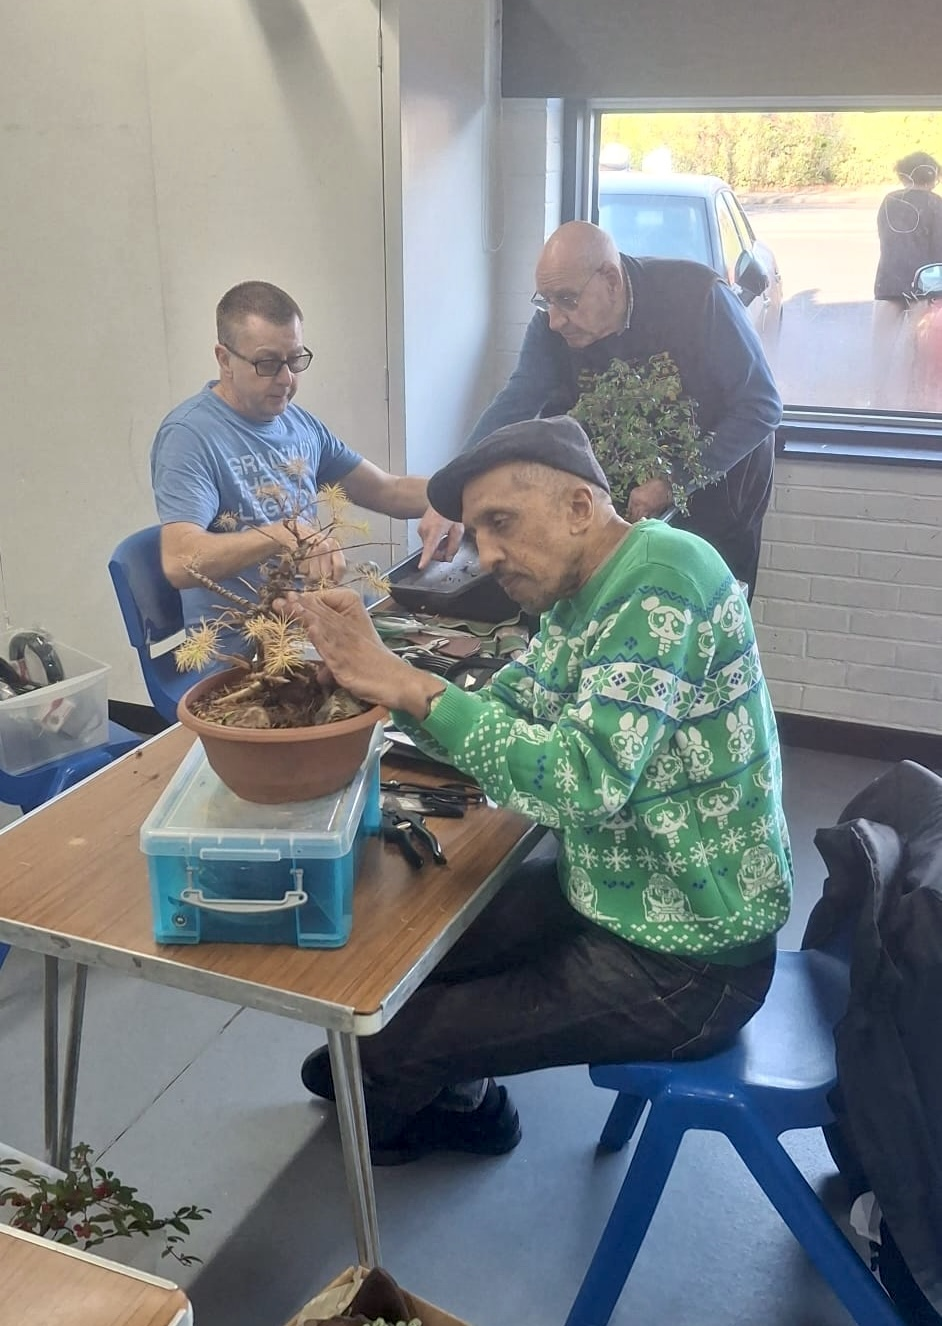
\includegraphics[angle=0,origin=c,width=1.0\textwidth]{2025_12/res/workshop-mep-wilson}
\centerline{\emph{Expert advice from Terry Wilson during the workshop.}}
\end{minipage}

\begin{minipage}[b]{0.45\textwidth}
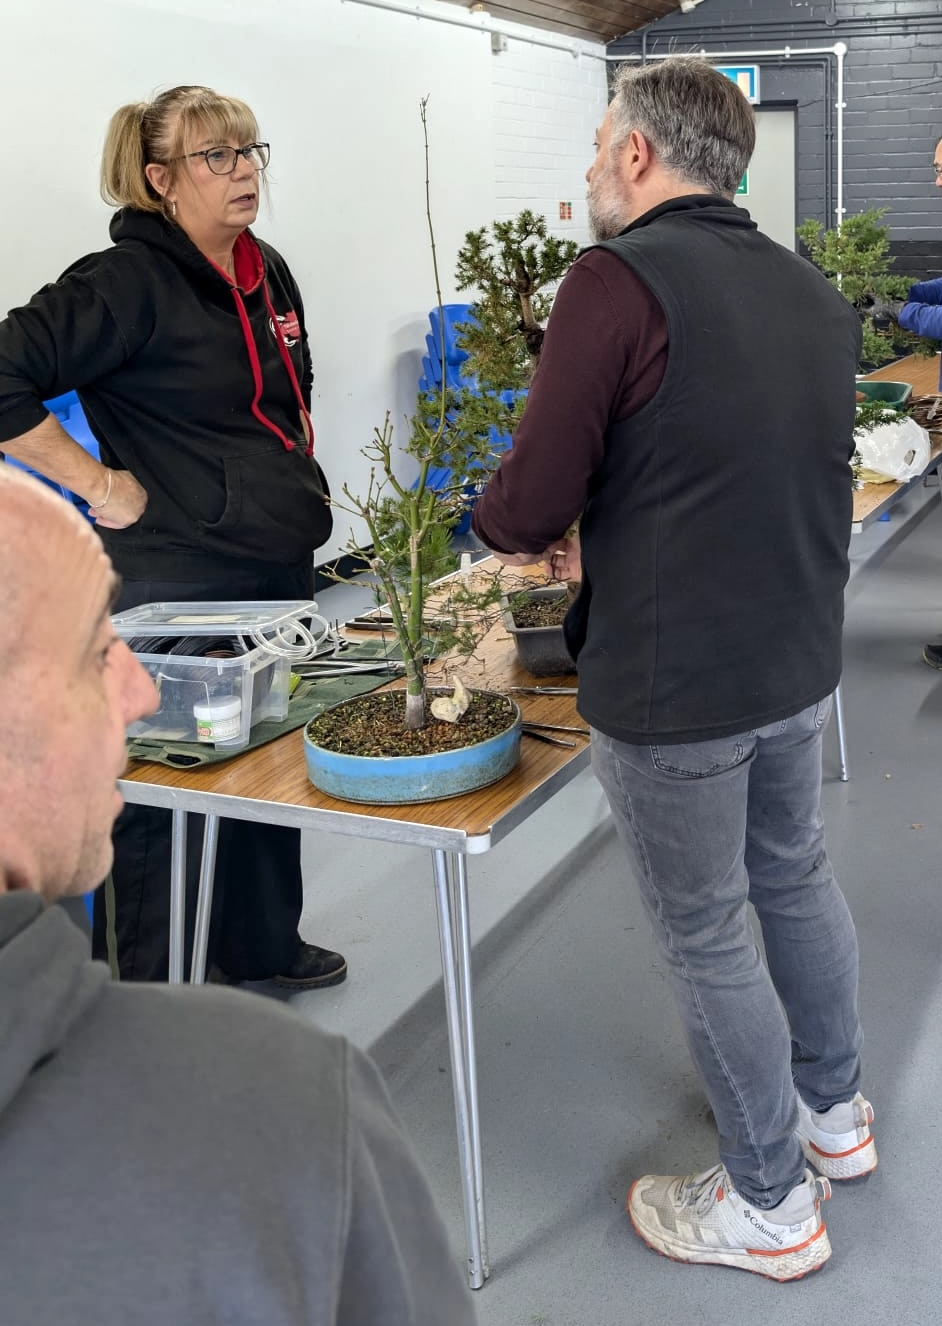
\includegraphics[angle=0,origin=c,width=1.0\textwidth]{2025_12/res/workshop-mep-todd}
\centerline{\emph{Tina Todd sharing her expertise with a fellow member.}}
\end{minipage}

\begin{minipage}[b]{0.45\textwidth}
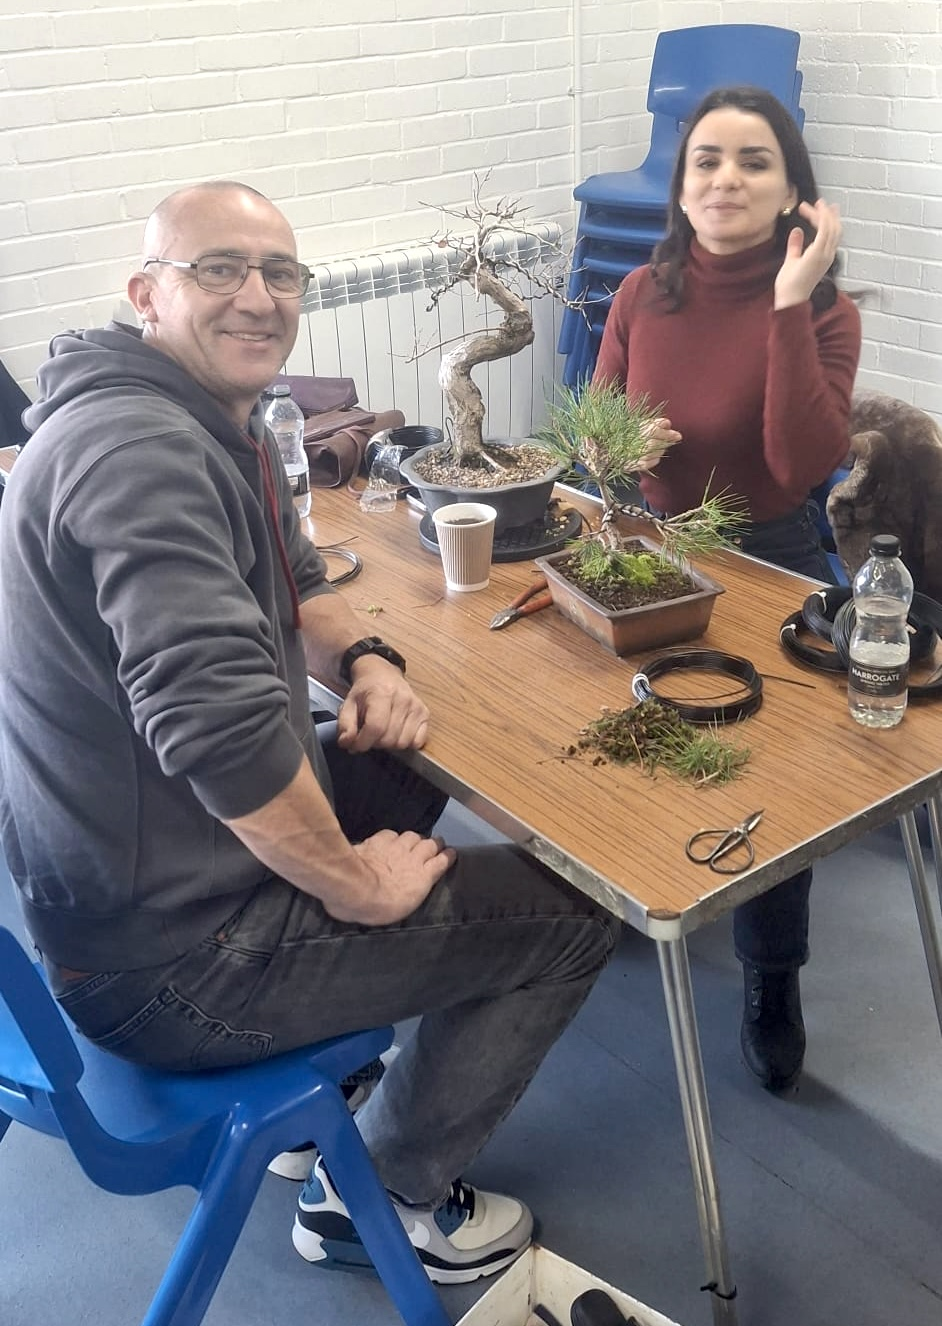
\includegraphics[angle=0,origin=c,width=1.0\textwidth]{2025_12/res/workshop-mep-members_1}
\centerline{\emph{Practicing new skills in a relaxed environment.}}
\end{minipage}

\begin{minipage}[b]{0.45\textwidth}
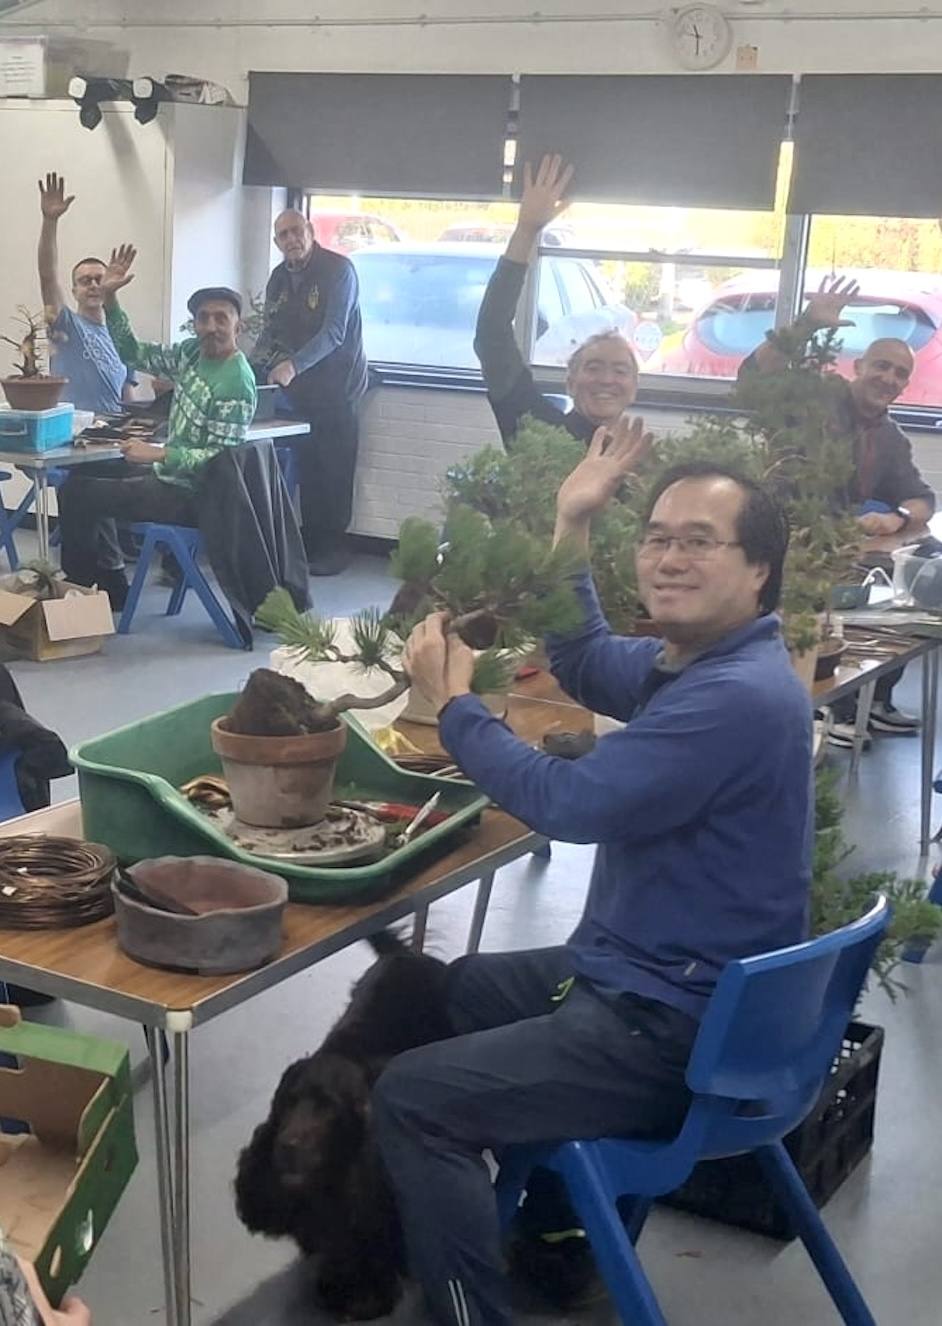
\includegraphics[angle=0,origin=c,width=1.0\textwidth]{2025_12/res/workshop-mep-members_2}
\centerline{\emph{Members gaining confidence during the session.}}
\end{minipage}

\columnbreak
